\documentclass[final]{beamer}
\mode<presentation>
{
  \usetheme{GCB}
}

\hyphenation{An-no-ta-tion-Sketch}

\usepackage{times,amsmath,amsthm,amssymb,latexsym,xspace}
\usepackage[english]{babel}
\usepackage[super]{nth}
\usepackage{textcomp}
\usepackage[utf8]{inputenc}
\usepackage[orientation=portrait,size=A0]{beamerposter}
\usepackage{ragged2e,sepnum,multicol}
% Display a grid to help align images
%\beamertemplategridbackground[1cm]
\bibliographystyle{apalike}
\setbeamertemplate{caption}[numbered]
\setbeamertemplate{items}[square]
%\setbeamertemplate{bibliography item}[text]

% some colors
\definecolor{arggrey}{gray}{.6}
\definecolor{middlegray}{gray}{.5}
\newcommand{\AnnotationSketch}{\emph{AnnotationSketch}\xspace}
\newcommand{\Gt}{\textit{GenomeTools}\xspace}

\title{\huge {\em LTRsift}: a graphical tool for semi-automatic classification and
       postprocessing of \emph{de novo} detected LTR retrotransposons}
\author[Steinbiss et al.]{Sascha Steinbiss, Sascha Kastens and Stefan Kurtz}
\institute[ZBH]{Research Group for Genome Informatics, Center for Bioinformatics, University of Hamburg, Hamburg, Germany}

\begin{document}

\begin{frame}[fragile]

  \begin{columns}[t]
    \begin{column}{.45\linewidth}

        \begin{block}{Homology-based vs.\ \emph{de novo} TE detection}
          \vspace{2mm}
          \begin{columns}
            \begin{column}{.4\linewidth}
             \alert{Homology-based tools}\\(e.g.\ RepeatMasker \cite{SMI:HUB:GRE:1996-2004})\\[.4cm]
             \begin{itemize}
              \item[+] high specificity
              \item[+] classification by match target
              \item[--] database availability?
              \item[--] bias towards known elements
              \item[--] opaque results: hit/no hit
             \end{itemize}
             \vspace{7mm}
            \end{column}
            \begin{column}{.5\linewidth}
            \alert{\emph{De novo} prediction tools}\\(e.g.\ LTR\_STRUC \cite{MCC:MCD:2003}, \emph{LTRharvest})\\[.3cm]
            \begin{itemize}
              \item[+] high sensitivity
              \item[+] database-independent
              \item[+] structured results
              \item[+] unknown elements can be detected
              \item[--] custom prediction tool for every repeat type
            \end{itemize}
            \vspace{.7cm}
          \end{column}
          \end{columns}
          \vspace{-.6cm}
        \end{block}

        \begin{block}{\emph{LTRharvest} and \emph{LTRdigest}}
          \centerline{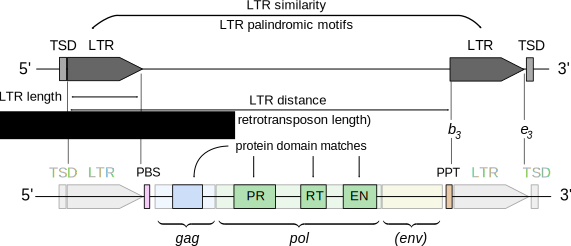
\includegraphics[width=.8\textwidth]{ltr}}
          \vspace{1.5cm}
          \begin{columns}
            \begin{column}{.45\linewidth}
              \alert{LTRharvest}~\cite{ELL:KUR:WIL:2008}
              \begin{itemize}
                \item index-based \emph{de novo} detection and annotation of
                      LTR retrotransposons
                \item \emph{LTRharvest} efficiently generates candidate pairs
                      of degenerate repeats from (possibly large) genomes,
                      e.g.\ whole mammalian genomes
                \item output: sequences, GFF3 annotations
              \end{itemize}
              \end{column}
            \begin{column}{.45\linewidth}
              \alert{LTRdigest}~\cite{STEI:WIL:GRE:KUR:2009}
              \begin{itemize}
                \item augments \emph{LTRharvest} output with additional
                      features present in a candidate's inner region
                \item PBS: local alignment to host tRNA
                \item PPT: base composition hidden Markov model
                \item functional domains: profile HMMs
              \end{itemize}
            \end{column}
          \end{columns}
        \end{block}

        \begin{block}{A \emph{de novo} library preparation workflow}
          \begin{columns}
            \begin{column}{.5\linewidth}
              \alert{Goal}\\
              generate a library of full-length reference sequences, typically
              one sequence per family\\
              \centerline{$\downarrow$}
              subsequent identification of incomplete insertions,
              solo LTRs, \dots\\[.5cm]
              \alert{Workflow}\\
              \begin{enumerate}
                \item obtain candidates with feature annotations
                \item filter out uninteresting candidates (e.g.\ without
                      protein domains, ORFs, \dots ) to separate file
                \item cluster features with similar sequences
                      using BLAST matches (result: cluster number)
                \item combine feature clusters to obtain putative families
                \item verify similarity of group members on a whole-sequence
                      level using multiple sequence alignment (MSA); discard
                      groups with less than 3 members or inconclusive MSA
                      results
                \item choose ``good'' representative sequences from each group
                      or determine consensus
              \end{enumerate}
              \end{column}
            \begin{column}{.4\linewidth}
              \begin{figure}
                \centerline{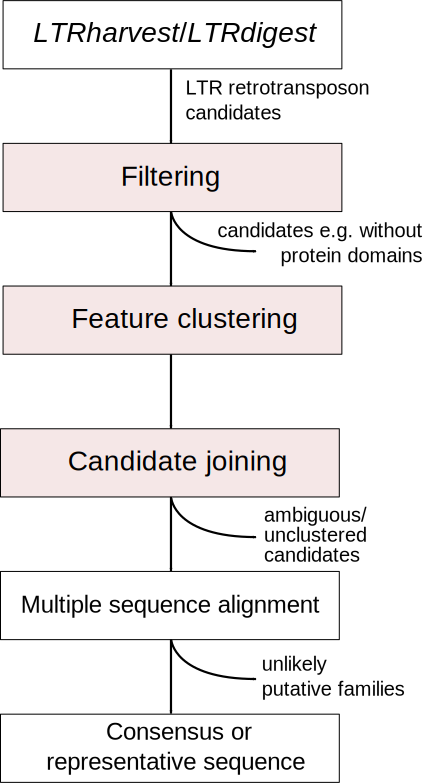
\includegraphics[width=.9\textwidth]{workflow}}
              \end{figure}
            \end{column}
          \end{columns}
        \end{block}


      \end{column}

   % right column
      \begin{column}{.45\linewidth}

        \begin{block}{Joining clustered candidates into groups}
          \begin{columns}
            \column{0.45\textwidth}
              \centerline{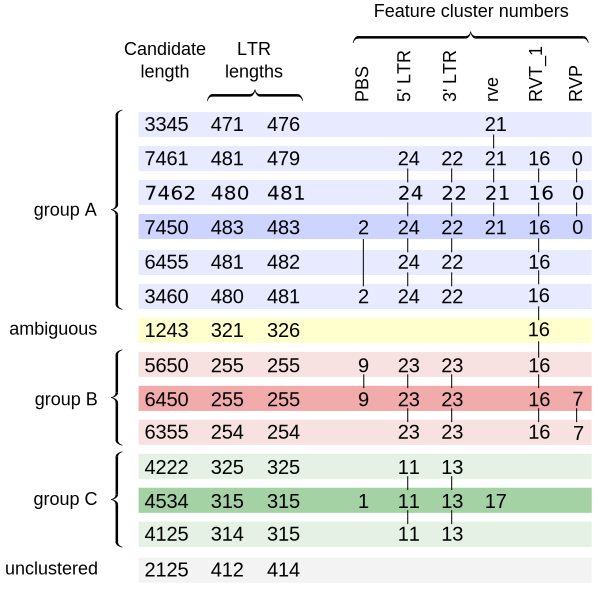
\includegraphics[width=\textwidth]{clusterjoining}}
            \column{0.45\textwidth}
              \alert{Compatibility}
              \begin{itemize}
                \item cluster numbers reflect similar feature sequences
                \item two candidates are \emph{compatible} iff their cluster
                      numbers do not contradict
              \end{itemize}
              \alert{Groups}
              \begin{itemize}
                \item \emph{groups} are maximal sets of candidates whose
                      members are pairwise compatible
                \item groups are regarded as \emph{putative families}
                \item select candidates in each group with most frequently
                      occurring features whose element and LTR lengths do not
                      deviate from the group median too much
                      $\to$ \emph{most complete} candidates
              \end{itemize}
          \end{columns}
        \end{block}

      \begin{block}{\emph{LTRsift} -- a graphical software tool to support
                    classification}
        \vspace{5mm}
        \begin{columns}
          \column{0.45\textwidth}
            \alert{Input}
            \begin{itemize}
              \item LTR retrotransposon candidate annotations in GFF3 format
              \item genomic sequences as \emph{encoded sequences}~\cite{STEI:KUR:2012}
            \end{itemize}
            \vspace{1cm}
          \column{0.45\textwidth}
            \alert{Output}
            \begin{itemize}
              \item annotations (GFF3) and sequences (FASTA) with putative
              family assignments for\dots
              \begin{itemize}
                \item all candidates (e.g.\ per family)
                \item filtered-out candidates
                \item most complete candidates
              \end{itemize}
            \end{itemize}
          \end{columns}
      \end{block}

      \begin{block}{Flexible definition of filtering rules}
        \begin{columns}
          \column{0.45\textwidth}
            \begin{itemize}
              \item candidates are represented as graphs
              \item \emph{nodes}: element features (LTRs, \dots)
                    \emph{edges}: \emph{part-of} relationships
              \item one candidate = one connected component (CC)
              \item filtering engine decides (true/false) for a
                    CC whether it is filtered or not
              \item filtered candidates are added to new families or unclassified
              \item rules can be defined in a simple programming language
            \end{itemize}
          \column{0.45\textwidth}
            \centerline{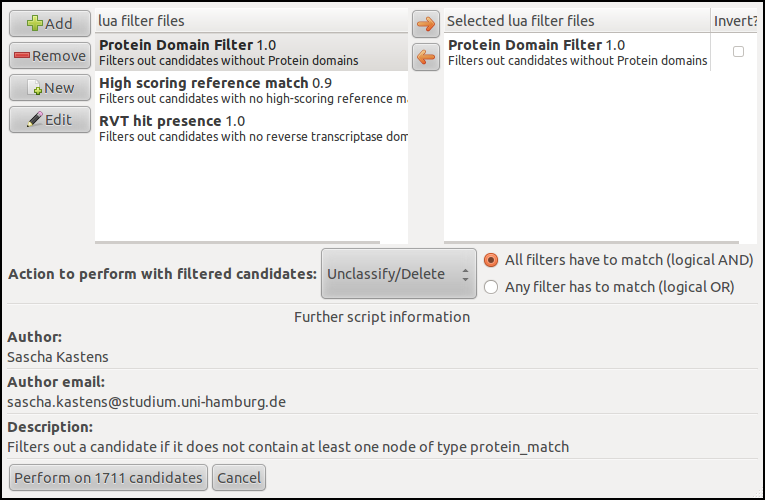
\includegraphics[width=\textwidth]{Graphics/screenshot_filter}}
          \end{columns}
      \end{block}

 \begin{columns}[t]
          \begin{column}{.45\linewidth}
           \vspace{-1cm}
              \begin{block}{Features}
                \begin{columns}
                  \column{.05\textwidth}
                  \column{.95\textwidth}
                    \begin{itemize}
                      \item wizard-guided project creation and
                            automated pre-classification
                      \item ``drag-and-drop'' manual family assignment
                      \item reference matching against custom FASTA files
                            (BLAST required)
                      \item ORF detection
                      \item concise, customizable visualization of\\
                            candidates~\cite{STEI:GRE:SCHAE:MAD:KUR:2009}
                      \item candidate lists can be sorted by column values
                      \item all project data stored in one\\persistent database
                      %\item no set-up necessary
                    \end{itemize}
                    \vspace{2mm}
                \end{columns}
            \end{block}
          \end{column}
          \begin{column}{.51\linewidth}
\vspace{-1.25cm}
            \begin{block}{Example: \emph{D.~melanogaster}}
              \begin{columns}
                  \column{.05\textwidth}
                  \column{.95\textwidth}
                    \alert{Goal}\\
                    reproduction of results from~\cite{STEI:WIL:GRE:KUR:2009}
                    \\[3mm]
                    \alert{Results}
                    \begin{itemize}
                      \item 714 candidates initially reported by
                            \emph{LTRharvest}/\emph{LTRdigest}
                      \item 318 candidates with PBS, 340 with PPT, 633 with protein domains
                      \item filtering and automatic classification:\\459
                            candidates in 52 putative families
                      \item 284 representative sequences, 44 of 52 families
                            recovered with $>80\,\%$ sequence similarity
                            compared to reference
                    \end{itemize}
                    \vspace{.60cm}
                \end{columns}
            \end{block}
          \end{column}
        \end{columns}

      \end{column}
    \end{columns}

\vspace{.6cm}

\begin{columns}[t]
     \column{.55\linewidth}
      \vspace{.5cm}
      \begin{center}
        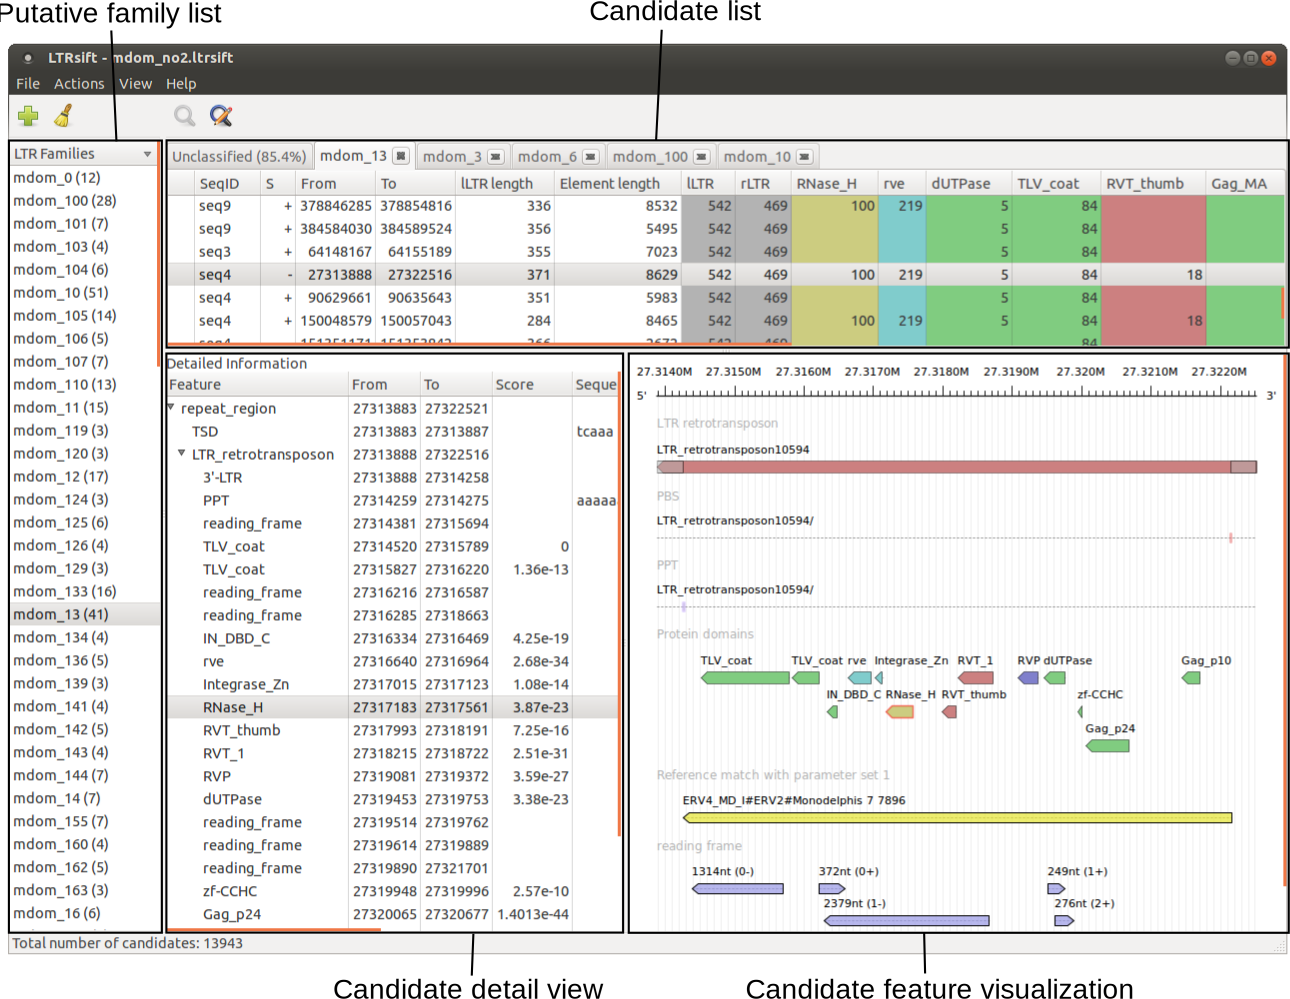
\includegraphics[width=.95\textwidth]{ltrsift_overview}
      \end{center}

     \column{.35\linewidth}

     \vspace{-4cm}
     \begin{block}{Example: \emph{Sus scrofa}}
        \begin{columns}
          \column{.45\textwidth}
            \alert{Goal}\\
            complete \emph{de novo} identification and family assignment
            of LTR retrotransposons in the pig genome\\[3mm]
            \alert{Results}
            \begin{itemize}
              \item \emph{LTRharvest}/\emph{LTRdigest} default
                    parameters, 14 Pfam domain models
              \item 2363 candidates initially reported and processed by
                    \emph{LTRharvest}/\emph{LTRdigest}
            \end{itemize}
          \column{.45\textwidth}
            \begin{itemize}
              \item 588 candidates with PBS, 967 with PPT, 125 with
                    protein domains
              \item automatic classification:\\291
                    candidates in 80 putative families
              \item prune unlikely families $\to$ 22 remaining families
              \item 17 representative sequences could be matched to
                    PERV-$\beta 3$, $\gamma 1$, $\gamma 2$ and $\gamma 7$
                    families with 89--100\,\% identity
            \end{itemize}
            \vspace{-1.5mm}
        \end{columns}
      \end{block}

      \begin{block}{Availability of the \emph{LTRsift} software}
        \begin{columns}
          \column{.02\textwidth}
          \column{.98\textwidth}
            \begin{itemize}
              \item free, open source software (GNU General Public License)
              \item based on the \emph{GenomeTools} toolkit~\cite{GRE:STEI:KUR:2012B}
              \item UNIX-like platforms (Linux, BSD, Mac OS X, \dots)
              \item available soon $\to$ \url{http://www.zbh.uni-hamburg.de/LTRsift}
            \end{itemize}
        \end{columns}
      \end{block}

       \begin{block}{References}
          \begin{scriptsize}
            \begin{multicols}{2}
              \bibliography{poster,ltr,kurtz}
            \end{multicols}
          \end{scriptsize}
        \end{block}
    \end{columns}

\end{frame}
\end{document}
